\chapter{Enemies and their Discontents} 
\label{sec:level}

\lstset{style=6502Style}

\begin{definition}[Jeffrey Says]
\setlength{\intextsep}{0pt}%
\setlength{\columnsep}{3pt}%
\begin{wrapfigure}{l}{0.12\textwidth}
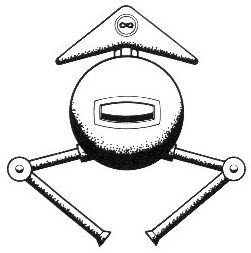
\includegraphics[width=\linewidth]{src/callout/ia.jpg} 
\end{wrapfigure}
\small
This is the bit that I knew would take me ages to write and get glitch
free, and the bit that is absolutely necessary to the functioning of the game.
The module ACONT is essentially an interpreter for my own 'wave language',
allowing me to describe, exactly, an attack wave in about 50 bytes of data. The
waves for the first part of IRIDIS are in good rollicking shoot-'em-up style,
and there have to be plenty of them. There are five planets and each planet\index{planet} is
to have twenty levels associated with it. It's impractical to write separate
bits of code for each wave; even with 64K you can run outta memory pretty fast
that way, and it's not really necessary coz a lot of stuff would be duplicated.
Hence ACONT.
\end{definition}

The bits and bytes that define the behaviour and appearance of
wave after wave of Iridis Alpha's enemy formations - twenty across each of the
five planets giving one hundred in all - take up relatively little space given
the sheer variety of adversaries the player faces.


\begin{figure}[H]
  {
    \setlength{\tabcolsep}{3.0pt}
    \setlength\cmidrulewidth{\heavyrulewidth} % Make cmidrule = 
	\begin{subfigure}{1\textwidth}
  \hspace{0.2cm}
    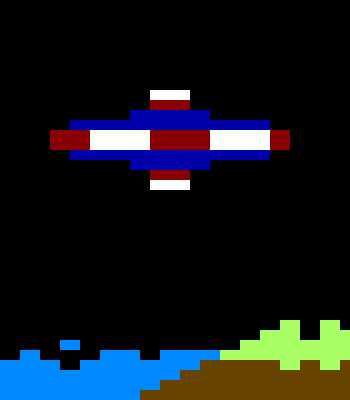
\includegraphics[width=3cm]{src/sprites/gallery/sprite_162.png}%
  \hspace{1.3cm}
    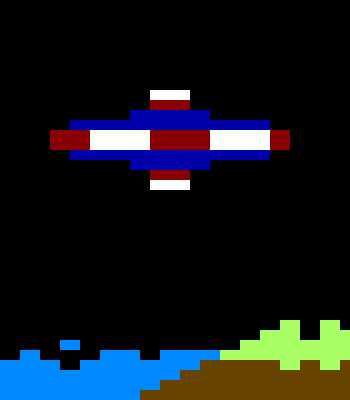
\includegraphics[width=3cm]{src/sprites/gallery/sprite_162.png}%
  \hspace{1.4cm}
    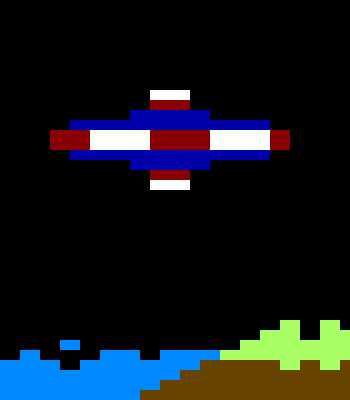
\includegraphics[width=3cm]{src/sprites/gallery/sprite_162.png}%
	\end{subfigure}
  }
  \vspace{1.4cm}

  {
  \setlength{\tabcolsep}{3.0pt}
  \setlength\cmidrulewidth{\heavyrulewidth} % Make cmidrule = 
  \begin{adjustbox}{width=13cm}

\begin{tabular}{lll}
\toprule
 Byte    & Value                     & Description                                                        \\
\midrule
 Byte 0     & \icode{\$06}                       & Index into array for sprite colour                                   \\
 Byte 1-2   & FLYING\_SAUCER1            & First and last sprite value for the attack ship on the upper planet\index{planet} \\
 Byte 3     & \icode{\$03}                       & The animation\index{animation} frame rate for the attack ship.                       \\
 Byte 4-5   & FLYING\_SAUCER1            & First and last sprite value for the attack ship on the lower planet\index{planet} \\
 Byte 6     & \icode{\$00}                       & Rate at which to switch to alternate enemy mode.                    \\
 Byte 7-8   & nullPtr\index{nullPtr}                   & Pointer for alternate enemy mode                                    \\
 Byte 9-10  & nullPtr\index{nullPtr}                   & Unused Pointer to an arbitrary run of Bytes 18-21.                  \\
 Byte 11    & \icode{\$00}                       & Unused Rate limit for use of Bytes 9 and 10.                        \\
 Byte 12-13 & nullPtr\index{nullPtr}                   & Unused Bytes                                                        \\
 Byte 14    & \icode{\$00}                       & Controls the rate at which new enemies\index{enemies} are added.                   \\
 Byte 15    & \icode{\$40}                       & Update rate for switching to the level data in Bytes 16/17          \\
 Byte 16-17 & planet1Level1Data2ndStage\index{planet1Level1Data2ndStage} & Pointer to wave data we switch to periodically.                     \\
 Byte 18    & \icode{\$06}                       & X Pos movement\index{movement} for attack ship.                                     \\
 Byte 19    & \icode{\$01}                       & Y Pos movement\index{movement} pattern\index{pattern} for attack ship.                             \\
 Byte 20    & \icode{\$01}                       & X Pos Frame Rate for Attack ship.                                   \\
 Byte 21    & \icode{\$01}                       & Y Pos Frame Rate for Attack ship.                                   \\
 Byte 22    & \icode{\$00}                       & Stickiness\index{Stickiness} factor, does the enemy stick to the player               \\
 Byte 23    & \icode{\$00}                       & Does the enemy gravitate quickly toward the player when its hit?    \\
 Byte 24-25 & nullPtr\index{nullPtr}                   & Pointer for second wave of attack ships.                            \\
 Byte 26-27 & nullPtr\index{nullPtr}                   & Pointer for third wave of attack ships.                             \\
 Byte 28-29 & spinningRings\index{spinningRings}             & Pointer for wave to switch to when hit by bullet.                   \\
 Byte 30-31 & defaultExplosion\index{defaultExplosion}          & Pointer for  wave to switch to after colliding\index{colliding} with gilby.          \\
 Byte 32-33 & \icode{\$00}                       & Pointer for fourth wave of attack ships.                            \\
 Byte 34    & \icode{\$02}                       & Points for hitting the enemy.                                       \\
 Byte 35    & \icode{\$02}                       & Energy increase multiplier for hitting an enemy.                    \\
 Byte 36    & \icode{\$00}                       & Is the ship a spinning\index{spinning} ring, i.e. does it allow the gilby to warp?  \\
 Byte 37    & \icode{\$04}                       & Number of waves in data.                                            \\
 Byte 38    & \icode{\$18}                       & Number of ships in wave.                                            \\
 Byte 39    & \icode{\$00}                       & Unused byte.                                                        \\
\bottomrule
\end{tabular}

  \end{adjustbox}

  }\caption{Sheep Planet - Level 1 - Enemy Data for the First Wave.}
\end{figure}
\clearpage

\section{Something Simple - Byte 0: The Enemy's Color}
To get an understanding of how the level data is used we can start with the very first byte of the data
used for the first wave in the very first level. This is the wave of flying saucers you will already be
familiar with if you have played the game:
\begin{figure}[H]
  {
    \setlength{\tabcolsep}{3.0pt}
    \setlength\cmidrulewidth{\heavyrulewidth} % Make cmidrule = 
	\centering
	\def\MULTICOLORONE{white}
	\def\MULTICOLORTWO{red}
	\def\SPRITECOLOR{blue}
	\begin{subfigure}{0.3\textwidth}
		\input{sprites/FLYING_SAUCER1}
	\end{subfigure}
	\begin{subfigure}{0.3\textwidth}
		\input{sprites/FLYING_SAUCER2}
	\end{subfigure}
	\begin{subfigure}{0.3\textwidth}
		\input{sprites/FLYING_SAUCER3}
	\end{subfigure}
  }\caption[position=top]{The sprites\index{sprites} used to animate the 'UFO' in the first level.}
\end{figure}

The main colour for this sprite is blue. This may not be obvious from looking at the sprites\index{sprites} themselves, but
the way the sprite colour schemes work is that you can select two colours that are available for all sprites\index{sprites} and
one colour that is unique to the sprite itself. In this case, the unique colour selected for the flying saucers is
determined by Byte 1 in the Level Data. You can see in the table in the page opposite
that this is defined with a value of \icode{\$06}. This is how it looks in the code itself:

\begin{lstlisting}[escapechar=\%]
planet1Level1Data%\index{planet1Level1Data}%
    ; Byte 0 (Index $00): An index into colorsForAttackShips%\index{colorsForAttackShips}% 
    ; that applies a colour value for the ship sprite.
    .BYTE $06
\end{lstlisting}

This value is an index into the array \icode{colorsForAttackShips\index{colorsForAttackShips}}. Starting at zero we count up to 6
and arrive at the 7th item in the list below, giving us the result \icode{BLUE}:
\begin{lstlisting}[escapechar=\%]
colorsForAttackShips%\index{colorsForAttackShips}%
    .BYTE BLACK,WHITE,RED,CYAN,PURPLE,GREEN,BLUE,YELLOW
    .BYTE ORANGE,BROWN,LTRED,GRAY1,GRAY2,LTGREEN%\index{LTGREEN}%,LTBLUE,GRAY3
\end{lstlisting}

In the routine\index{routine} that draws the attack wave we find the following code segment writing this value
to the register\index{register} \icode{\$D027} that determines the colour of the sprite:

\begin{lstlisting}[escapechar=\%]
DrawUpperPlanetAttackShips%\index{DrawUpperPlanetAttackShips}%
    LDX #$0C
    LDY #$06
UpperPlanetShipsLoop%\index{UpperPlanetShipsLoop}%   
    ...
    LDX upperPlanetAttackShipsColorArray%\index{upperPlanetAttackShipsColorArray}%,Y
    LDA colorsForAttackShips%\index{colorsForAttackShips}%,X
    STA $D027,Y  ;Sprite Y Color
    ...
    DEX
    DEX
    DEY
    BNE UpperPlanetShipsLoop%\index{UpperPlanetShipsLoop}%
    RTS
\end{lstlisting}

Notice that the \icode{\$06} was originally stored in a position in the array \icode{upperPlanet\-AttackShipsColorArray}.
This happened in an earlier routine\index{routine} that loads the majority of the data for a level:


\begin{lstlisting}[escapechar=\%]
GetWaveDataForNewShip%\index{GetWaveDataForNewShip}%
    ; X is the index of the ship in activeShipsWaveDataLoPtrArray%\index{activeShipsWaveDataLoPtrArray}%
    LDY #$00
    LDA (currentShipWaveDataLoPtr%\index{currentShipWaveDataLoPtr}%),Y
    STA upperPlanetAttackShipsColorArray%\index{upperPlanetAttackShipsColorArray}% + $01,X
\end{lstlisting}

\section{Bytes 1-4: Sprite Animation}
\begin{definition}[Jeffrey Says]
\setlength{\intextsep}{0pt}%
\setlength{\columnsep}{3pt}%
\begin{wrapfigure}{l}{0.12\textwidth}
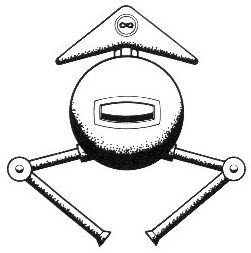
\includegraphics[width=\linewidth]{src/callout/ia.jpg} 
\end{wrapfigure}
\small
You pass the interpreter data, that describes exactly stuff like: what each
alien looks like, how many frames of animation\index{animation} it uses, speed of that
animation\index{animation}, colour, velocities\index{velocities} in X— and Y— directions, accelerations\index{accelerations} in X and
Y, whether the alien should 'home in' on a target, and if so, what to home in
on; whether an alien is subject to gravity\index{gravity}, and if so, how strong is the
gravity\index{gravity}; what the alien should do if it hits top of screen\index{screen}, the ground, one of
your bullets\index{bullets}, or you; whether the alien can fire bullets\index{bullets}, and if so, how
frequently, and what types; how many points you get if you shoot it, and how
much damage it does if it hits you; and a whole bunch more stuff like that. As
you can imagine it was a fairly heavy routine\index{routine} to write and get debugged\index{debugged}, but
that's done now; took me about three weeks in all I'd say.
\end{definition}

\begin{figure}[H]
  {
    \setlength{\tabcolsep}{3.0pt}
    \setlength\cmidrulewidth{\heavyrulewidth} % Make cmidrule = 
	\centering
	\def\MULTICOLORONE{red}
	\def\MULTICOLORTWO{white}
	\def\SPRITECOLOR{orange}
	\begin{subfigure}{0.3\textwidth}
		\input{sprites/CUMMING_COCK1}
	\end{subfigure}
	\begin{subfigure}{0.3\textwidth}
		\input{sprites/CUMMING_COCK2}
	\end{subfigure}
	\begin{subfigure}{0.3\textwidth}
		\input{sprites/CUMMING_COCK3}
	\end{subfigure}
  }\caption[position=top]{Confirmation that the game developer was a young caucasian male. The sprites\index{sprites} used to animate attack wave 17 in the Mushroom Planet.}
\end{figure}

Looking again at the table in the previous page we can see the first 7 bytes are concerned with the appearance and basic behaviour of the
enemy. Bytes 1 and 2 define the sprite used for display on the upper planet\index{planet}, Bytes 4 and 5
for the lower planet\index{planet}. The reason there's two in each case is because they are describing the
start and end point of the sprite's animation\index{animation}. 

We can see this in action in \icode{AnimateAttackShipSprites\index{AnimateAttackShipSprites}}. When this routine\index{routine} runs Byte 3 has been loaded
to \icode{upperPlanetAttackShipInitialFrameRate\index{upperPlanetAttackShipInitialFrameRate}} for the upper planet\index{planet} and \icode{lowerPlanetAttackShipInitialFrameRate\index{lowerPlanetAttackShipInitialFrameRate}}
for the lower planet\index{planet}. This routine\index{routine} is cycling through the sprites\index{sprites} given by Byte 1 as the lower limit and Byte 2 as 
the upper limit. This is what the animation\index{animation} consists of: changing the sprite from
one to another to create a classic animation\index{animation} effect.

\begin{lstlisting}[caption=Routine for Animating Enemy Sprites\index{Sprites}. ,escapechar=\%]
AnimateAttackShipSprites%\index{AnimateAttackShipSprites}%
    LDA pauseModeSelected%\index{pauseModeSelected}%
    BEQ AnimateUpperPlanetAttackShips%\index{AnimateUpperPlanetAttackShips}%
    RTS

AnimateUpperPlanetAttackShips%\index{AnimateUpperPlanetAttackShips}%   
    DEC upperPlanetAttackShipAnimationFrameRate%\index{upperPlanetAttackShipAnimationFrameRate}% - $01,X
    BNE AnimateLowerPlanetAttackShips%\index{AnimateLowerPlanetAttackShips}%

    LDA upperPlanetAttackShipInitialFrameRate%\index{upperPlanetAttackShipInitialFrameRate}% - $01,X
    STA upperPlanetAttackShipAnimationFrameRate%\index{upperPlanetAttackShipAnimationFrameRate}% - $01,X
    INC upperPlanetAttackShip2SpriteValue%\index{upperPlanetAttackShip2SpriteValue}%,X
    LDA upperPlanetAttackShip2SpriteValue%\index{upperPlanetAttackShip2SpriteValue}%,X

    ; Reached%\index{Reached}% the end of the animation%\index{animation}%?
    CMP upperPlanetAttackShipSpriteAnimationEnd%\index{upperPlanetAttackShipSpriteAnimationEnd}% - $01,X
    BNE AnimateLowerPlanetAttackShips%\index{AnimateLowerPlanetAttackShips}%

    ; Reset the animation%\index{animation}% sprite back to the start.
    LDA upperPlanetAttackShipSpritesLoadedFromBackingData - $01,X
    STA upperPlanetAttackShip2SpriteValue%\index{upperPlanetAttackShip2SpriteValue}%,X

AnimateLowerPlanetAttackShips%\index{AnimateLowerPlanetAttackShips}%   
    DEC lowerPlanetAttackShipAnimationFrameRate%\index{lowerPlanetAttackShipAnimationFrameRate}% - $01,X
    BNE DontAnimateLowerPlanetAttackShip%\index{DontAnimateLowerPlanetAttackShip}%

    LDA lowerPlanetAttackShipInitialFrameRate%\index{lowerPlanetAttackShipInitialFrameRate}% - $01,X
    STA lowerPlanetAttackShipAnimationFrameRate%\index{lowerPlanetAttackShipAnimationFrameRate}% - $01,X
    INC lowerPlanetAttackShip2SpriteValue%\index{lowerPlanetAttackShip2SpriteValue}%,X
    LDA lowerPlanetAttackShip2SpriteValue%\index{lowerPlanetAttackShip2SpriteValue}%,X

    ; Reached%\index{Reached}% the end of the animation%\index{animation}%?
    CMP lowerPlanetAttackShipSpriteAnimationEnd%\index{lowerPlanetAttackShipSpriteAnimationEnd}% - $01,X
    BNE DontAnimateLowerPlanetAttackShip%\index{DontAnimateLowerPlanetAttackShip}%

    ; Reset the animation%\index{animation}% sprite back to the start.
    LDA lowerPlanetAttackShipSpritesLoadedFromBackingData - $01,X
    STA lowerPlanetAttackShip2SpriteValue%\index{lowerPlanetAttackShip2SpriteValue}%,X
DontAnimateLowerPlanetAttackShip%\index{DontAnimateLowerPlanetAttackShip}%   
    RTS
\end{lstlisting}
 
Byte 1 (loaded to \icode{upperPlanetAttackShipAnimationFrameRate\index{upperPlanetAttackShipAnimationFrameRate}} comes into play here. It's decremented and as long as it's
not zero yet the animation\index{animation} is skipped, execution jumps forward to \icode{AnimateLowerPlanetAttackShips\index{AnimateLowerPlanetAttackShips}}:

\begin{lstlisting}[escapechar=\%]
AnimateLowerPlanetAttackShips%\index{AnimateLowerPlanetAttackShips}%   
    DEC lowerPlanetAttackShipAnimationFrameRate%\index{lowerPlanetAttackShipAnimationFrameRate}% - $01,X
    BNE DontAnimateLowerPlanetAttackShip%\index{DontAnimateLowerPlanetAttackShip}%

    LDA lowerPlanetAttackShipInitialFrameRate%\index{lowerPlanetAttackShipInitialFrameRate}% - $01,X
    STA lowerPlanetAttackShipAnimationFrameRate%\index{lowerPlanetAttackShipAnimationFrameRate}% - $01,X
    INC lowerPlanetAttackShip2SpriteValue%\index{lowerPlanetAttackShip2SpriteValue}%,X
    LDA lowerPlanetAttackShip2SpriteValue%\index{lowerPlanetAttackShip2SpriteValue}%,X

    ; Reached%\index{Reached}% the end of the animation%\index{animation}%?
    CMP lowerPlanetAttackShipSpriteAnimationEnd%\index{lowerPlanetAttackShipSpriteAnimationEnd}% - $01,X
    BNE DontAnimateLowerPlanetAttackShip%\index{DontAnimateLowerPlanetAttackShip}%

    ; Reset the animation%\index{animation}% sprite back to the start.
    LDA lowerPlanetAttackShipSpritesLoadedFromBackingData - $01,X
    STA lowerPlanetAttackShip2SpriteValue%\index{lowerPlanetAttackShip2SpriteValue}%,X
\end{lstlisting}

If it is zero, it instead gets reset to the initial value from Byte 1 (stored in
 \icode{upperPlanet\-AttackShipInitialFrameRate})
and the current sprite for the enemy ship is incremented to point to the next 'frame' of the ship's animation\index{animation}:

\begin{lstlisting}[escapechar=\%]
AnimateUpperPlanetAttackShips%\index{AnimateUpperPlanetAttackShips}%   
    DEC upperPlanetAttackShipAnimationFrameRate%\index{upperPlanetAttackShipAnimationFrameRate}% - $01,X
    BNE AnimateLowerPlanetAttackShips%\index{AnimateLowerPlanetAttackShips}%

    LDA upperPlanetAttackShipInitialFrameRate%\index{upperPlanetAttackShipInitialFrameRate}% - $01,X
    STA upperPlanetAttackShipAnimationFrameRate%\index{upperPlanetAttackShipAnimationFrameRate}% - $01,X
    INC upperPlanetAttackShip2SpriteValue%\index{upperPlanetAttackShip2SpriteValue}%,X
    LDA upperPlanetAttackShip2SpriteValue%\index{upperPlanetAttackShip2SpriteValue}%,X

    ; Reached%\index{Reached}% the end of the animation%\index{animation}%?
    CMP upperPlanetAttackShipSpriteAnimationEnd%\index{upperPlanetAttackShipSpriteAnimationEnd}% - $01,X
    BNE AnimateLowerPlanetAttackShips%\index{AnimateLowerPlanetAttackShips}%

    ; Reset the animation%\index{animation}% sprite back to the start.
    LDA upperPlanetAttackShipSpritesLoadedFromBackingData - $01,X
    STA upperPlanetAttackShip2SpriteValue%\index{upperPlanetAttackShip2SpriteValue}%,X
\end{lstlisting}

Next we check if we've reached the end of the animation\index{animation} by checking the value
of Byte 2 (loaded to \icode{upperPlanetAttackShipSpriteAnimationEnd\index{upperPlanetAttackShipSpriteAnimationEnd}}).  If so,
we reset \icode{upperPlanetAttackShip2SpriteValue\index{upperPlanetAttackShip2SpriteValue}} to the value initially
loaded from Byte 1 - and that is what will be used to display the ship the next
time we pass through to animate the ship:

\begin{lstlisting}[escapechar=\%]
DrawUpperPlanetAttackShips%\index{DrawUpperPlanetAttackShips}%
    LDX #$0C
    LDY #$06
UpperPlanetShipsLoop%\index{UpperPlanetShipsLoop}%   
    LDA upperPlanetAttackShipsXPosArray%\index{upperPlanetAttackShipsXPosArray}%,Y
    STA $D000,X  ;Sprite 0 X Pos

    LDA attackShipsXPosArray%\index{attackShipsXPosArray}% - $01,Y
    AND $D010    ;Sprites%\index{Sprites}% 0-7 MSB of X coordinate
    STA currentMSBXPosOffset%\index{currentMSBXPosOffset}%

    LDA upperPlanetAttackShipsMSBXPosArray%\index{upperPlanetAttackShipsMSBXPosArray}%,Y
    AND attackShipsMSBXPosOffsetArray%\index{attackShipsMSBXPosOffsetArray}%,Y
    ORA currentMSBXPosOffset%\index{currentMSBXPosOffset}%
    STA $D010    ;Sprites%\index{Sprites}% 0-7 MSB of X coordinate

    LDA upperPlanetAttackShipsYPosArray%\index{upperPlanetAttackShipsYPosArray}%,Y
    STA $D001,X  ;Sprite 0 Y Pos
    STX tempVarStorage%\index{tempVarStorage}%

    LDX upperPlanetAttackShipsColorArray%\index{upperPlanetAttackShipsColorArray}%,Y
    LDA colorsForAttackShips%\index{colorsForAttackShips}%,X
    STA $D027,Y  ;Sprite 0 Color

    LDA upperPlanetAttackShipsSpriteValueArray%\index{upperPlanetAttackShipsSpriteValueArray}%,Y
    STA Sprite0Ptr%\index{Sprite0Ptr}%,Y
    LDX tempVarStorage%\index{tempVarStorage}%

    DEX
    DEX
    DEY
    BNE UpperPlanetShipsLoop%\index{UpperPlanetShipsLoop}%
    RTS
\end{lstlisting}

\section{Bytes 18-21: Enemy Movement}

Enemy movement\index{movement} is controlled by two parameters in each direction: the number of pixels to move in one go and the number of
cycles to wait between each movement\index{movement}. So for movement\index{movement} in the horizontal (or X direction) \icode{Byte 18} controls the number
of pixels to move at once, while \icode{Byte 20} controls the number of cycles to wait between each movement\index{movement}. The same
applies to \icode{Byte 19} and \icode{Byte 21} for the vertical (or Y direction).

If we look at Byte 18 and Byte 20 for Level 1 we can see that the the fast lateral movement\index{movement} of the 'UFO's is implemented by a relatively
high value of \$06 for the number of pixels it moves at each step while the interval between steps is relatively low (\$01).
Meanwhile the more gradual up and down movement\index{movement} is implemented by a value of \$01 in Byte 19 and Byte 21.

For the second level ('bouncing rings') the horizontal movement\index{movement} is more constrained (Byte 18 is \$00) while the vertical movement\index{movement}
is more extreme (Byte 19 is \$24) - achieving the bouncing effect.



\begin{figure}[H]
  {
    \setlength{\tabcolsep}{3.0pt}
    \setlength\cmidrulewidth{\heavyrulewidth} % Make cmidrule = 
    \begin{adjustbox}{width=8cm,center}

      \begin{tabular}{rlllll}
        \toprule
        Level & Byte 6    & Byte 18   & Byte 19   & Byte 20   & Byte 21   \\
        \midrule
        1 & \$00       & \$06       & \$01       & \$01       & \$01       \\
        2 & \$00       & \$00       & \$24       & \$02       & \$01       \\
        3 & \$00       & \$FA       & \$01       & \$01       & \$02       \\
        \addlinespace
        \bottomrule
        \multicolumn{6}{@{}l@{}}{Byte 6 : Whether a specific attack behaviour is used.}\\
        \multicolumn{6}{@{}l@{}}{Byte 18: X Pos movement\index{movement} for attack ship.}\\
        \multicolumn{6}{@{}l@{}}{Byte 19: Y Pos movement\index{movement} pattern\index{pattern} for attack ship.}\\
        \multicolumn{6}{@{}l@{}}{Byte 20: X Pos Frame Rate for Attack ship.}\\
        \multicolumn{6}{@{}l@{}}{Byte 21: Y Pos Frame Rate for Attack ship.}\\
      \end{tabular}

    \end{adjustbox}

    }\caption{Movement data for the first three levels.}
\end{figure}

The horizontal movement\index{movement} for Level Three, home to the infamous 'Licker Ships' is \$FA, which would make you think the enemies\index{enemies} must be moving horizontally
extremely quickly. In fact, when the high bit is set a special behaviour is invoked:

\begin{lstlisting}[caption=From \icode{UpdateAttackShipsXAndYPositions\index{UpdateAttackShipsXAndYPositions}}.  ,escapechar=\%]
        LDA xPosMovementForUpperPlanetAttackShip%\index{xPosMovementForUpperPlanetAttackShip}% - $01,X
        BMI UpperBitSetOnXPosMovement%\index{UpperBitSetOnXPosMovement}%
\end{lstlisting}

This is the special behaviour that makes the Licker Ships on this level such an enormous pain in the arse to play against.

\begin{figure}[H]
    \centering
    \foreach \l in {0,...,1}
    {
      \includegraphics[width=6cm]{level_data/images/movement_1_3_\l.png}%
    }%
\caption{Enemy movement\index{movement} for Sheep planet\index{planet}, level 3 - the infamous licker ships.}
\end{figure}

When the upper bit is set (e.g. \$FC,\$80) on the value loaded to the accumulator by \icode{LDA} then \icode{BMI} will 
return true and jump to \icode{UpperBitSetOnXPosMovement\index{UpperBitSetOnXPosMovement}}.

\begin{lstlisting}[escapechar=\%]
UpperBitSetOnXPosMovement%\index{UpperBitSetOnXPosMovement}%   
        ; This creates a decelerating%\index{decelerating}% effect on the attack ship's movement%\index{movement}%.
        ; Used by the licker ship wave in planet%\index{planet}% 1 for example.
        EOR #$FF
        STA attackShipOffsetRate%\index{attackShipOffsetRate}%
        INC attackShipOffsetRate%\index{attackShipOffsetRate}%
        LDA upperPlanetAttackShip2XPos%\index{upperPlanetAttackShip2XPos}%,X
        SEC
        SBC attackShipOffsetRate%\index{attackShipOffsetRate}%
        STA upperPlanetAttackShip2XPos%\index{upperPlanetAttackShip2XPos}%,X
        BCS DecrementXPosFrameRateLowerPlanet%\index{DecrementXPosFrameRateLowerPlanet}%

        LDA upperPlanetAttackShip2MSBXPosValue%\index{upperPlanetAttackShip2MSBXPosValue}%,X
        EOR attackShip2MSBXPosOffsetArray%\index{attackShip2MSBXPosOffsetArray}%,X
        STA upperPlanetAttackShip2MSBXPosValue%\index{upperPlanetAttackShip2MSBXPosValue}%,X
\end{lstlisting}

This first line \icode{EOR \#\$FF} performs an exclusive-or between Byte 19 in the \icode{Accumulator} (\$FA) and the value \$FF. An exclusive-or,
remember, is a bit by bit comparison of two bytes which will set a bit in the result if an only if the bit in one of the
values is set but the other is not:

\begin{figure}[H]
  {
    \setlength{\tabcolsep}{3.0pt}
    \setlength\cmidrulewidth{\heavyrulewidth} % Make cmidrule = 
    \begin{adjustbox}{width=7cm,center}

      \begin{tabular}{rllllllll}
        \toprule
        Byte & Bit 7 & Bit 6 & Bit 5 & Bit 4 & Bit 3 & Bit 2 & Bit 1 & Bit 0        \\
        \midrule
        \$FF & 1 & 1 & 1 & 1 & 1 & 1 & 1 & 1 \\
        \$FA & 1 & 1 & 1 & 1 & 1 & 0 & 1 & 0 \\
        \midrule
        Result & 0 & 0 & 0 & 0 & 0 & 1 & 0 & 1 \\
        \addlinespace
        \bottomrule
      \end{tabular}

    \end{adjustbox}

    }\caption*{X-OR'ing \$FF and \$FA gives \$05.}
\end{figure}

This result is stored in \icode{attackShipOffsetRate\index{attackShipOffsetRate}}:
\begin{lstlisting}[escapechar=\%]
UpperBitSetOnXPosMovement%\index{UpperBitSetOnXPosMovement}%   
  ; This creates a decelerating%\index{decelerating}% effect on the attack ship's movement%\index{movement}%.
  ; Used by the licker ship wave in planet%\index{planet}% 1 for example.
  EOR #$FF
  STA attackShipOffsetRate%\index{attackShipOffsetRate}%
\end{lstlisting}

Incremented:
\begin{lstlisting}[escapechar=\%]
        INC attackShipOffsetRate%\index{attackShipOffsetRate}%
\end{lstlisting}

And then subtracted from the enemy's X position:
\begin{lstlisting}[escapechar=\%]
  SEC
  SBC attackShipOffsetRate%\index{attackShipOffsetRate}%
  STA upperPlanetAttackShip2XPos%\index{upperPlanetAttackShip2XPos}%,X
\end{lstlisting}

The net result is a deceleration effect. This is observed in the way the licker ship
wave will accelerate out to the center before dialling back again.


\subsection{What is going on with Byte 6?}

Byte 6 comes into play when setting the initial Y position of a new enemy. This initial vertical
position is random, but subject to some adjustment:

\begin{lstlisting}[caption=The sub-routine\index{routine} \icode{SetInitialRandomPositionUpperPlanet\index{SetInitialRandomPositionUpperPlanet}} in \icode{GetWaveDateForNewShip\index{GetWaveDateForNewShip}}.  ,escapechar=\%]
SetInitialRandomPositionUpperPlanet%\index{SetInitialRandomPositionUpperPlanet}%   
  JSR PutProceduralByteInAccumulatorRegister%\index{PutProceduralByteInAccumulatorRegister}%
  AND #$3F
  CLC
  ADC #$40
  STA upperPlanetAttackShipsYPosArray%\index{upperPlanetAttackShipsYPosArray}% + $01,Y

  STY previousAttackShipIndexTmp%\index{previousAttackShipIndexTmp}%
  ; Byte 6 ($06): Usually an update rate for the attack ships.
  LDY #$06
  LDA (currentShipWaveDataLoPtr%\index{currentShipWaveDataLoPtr}%),Y
  BNE ReturnFromLoadingWaveDataEarly%\index{ReturnFromLoadingWaveDataEarly}%

  ; Byte 8 ($08): Default initiation%\index{initiation}% Y position for the enemy. 
  LDY #$08
  LDA (currentShipWaveDataLoPtr%\index{currentShipWaveDataLoPtr}%),Y
  BEQ ReturnFromLoadingWaveDataEarly%\index{ReturnFromLoadingWaveDataEarly}%

  LDA #$6C
  LDY previousAttackShipIndexTmp%\index{previousAttackShipIndexTmp}%
  STA upperPlanetAttackShipsYPosArray%\index{upperPlanetAttackShipsYPosArray}% + $01,Y

ReturnFromLoadingWaveDataEarly%\index{ReturnFromLoadingWaveDataEarly}%   
  RTS
\end{lstlisting}

The first order of business is to call \icode{PutProceduralByteInAccumulatorRegister\index{PutProceduralByteInAccumulatorRegister}} which gets a random value and stores it in the accumulator.

\begin{lstlisting}[escapechar=\%]
PutProceduralByteInAccumulatorRegister%\index{PutProceduralByteInAccumulatorRegister}%
randomIntToIncrement%\index{randomIntToIncrement}%   =*+$01
    LDA randomPlanetData%\index{randomPlanetData}%
    INC randomIntToIncrement%\index{randomIntToIncrement}%
    RTS
\end{lstlisting}

Since \icode{A} can now contain anything from 0 to 255 (\$00 to \$FF) this needs to be adjusted to a meaningful Y-position
value for the upper planet\index{planet}. So if we imagine \icode{PutProceduralByteInAccumulatorRegister\index{PutProceduralByteInAccumulatorRegister}} returned \$85, we now do the
following operations on it:

\begin{lstlisting}[escapechar=\%]
        AND #$3F
        CLC
        ADC #$40
        STA upperPlanetAttackShipsYPosArray%\index{upperPlanetAttackShipsYPosArray}% + $01,Y
\end{lstlisting}

First we do an \icode{AND \#\$3F} with the value of \$85 in \icode{A}:
\begin{figure}[H]
  {
    \setlength{\tabcolsep}{3.0pt}
    \setlength\cmidrulewidth{\heavyrulewidth} % Make cmidrule = 
    \begin{adjustbox}{width=7cm,center}

      \begin{tabular}{rllllllll}
        \toprule
        Byte & Bit 7 & Bit 6 & Bit 5 & Bit 4 & Bit 3 & Bit 2 & Bit 1 & Bit 0        \\
        \midrule
        \$85 & 1 & 0 & 0 & 0 & 0 & 1 & 0 & 1 \\
        \$3F & 0 & 0 & 1 & 1 & 1 & 1 & 1 & 1 \\
        \midrule
        Result & 0 & 0 & 0 & 0 & 0 & 1 & 0 & 1 \\
        \addlinespace
        \bottomrule
      \end{tabular}

    \end{adjustbox}

    }\caption*{AND'ing \$3F and \$85 gives \$05.}
\end{figure}

Our result is \$05. The effect of the AND'ing here is to ensure that the random number we get back is between 0 and 63 rather
than 0 and 255. Next we add \$40 (decimal\index{decimal} 64) to this result:

\begin{lstlisting}[escapechar=\%]
        CLC
        ADC #$40
\end{lstlisting}

This gives \$45 and this is what we store as the initial Y position for the enemy.

You'll notice that the steps for \icode{SetInitialRandomPositionLowerPlanet\index{SetInitialRandomPositionLowerPlanet}} are identical but with only the constant of the
add value of \$98 instead of \$40. This is simply an additional offset to ensure that the Y position is lower on the screen\index{screen}
for the initial position of the enemy on the lower planet\index{planet}.

We still haven't got into what Byte 7 is doing though. With an initial Y position determined, it looks like the intention was
for Byte 6 to specify some adjustment to this value. But this looks like another bit of non-functioning game logic. If
Byte 6 contains a value, the function\index{function} will return early without any further adjustments. If it's zero it will then try
Byte 8. If that's zero, it will return early. So the logic needs Byte 6 to be zero and Byte 8 to contain something for 
anything to happen. That's never the case, so the the adjustment never happens:

\begin{lstlisting}[caption= An adjustment that never happens. Byte 6 and Byte 8 are never set in this way.,escapechar=\%]
        STY previousAttackShipIndexTmp%\index{previousAttackShipIndexTmp}%
        ; Byte 6 ($06): Usually an update rate for the attack ships.
        LDY #$06
        LDA (currentShipWaveDataLoPtr%\index{currentShipWaveDataLoPtr}%),Y
        BNE ReturnFromLoadingWaveDataEarly%\index{ReturnFromLoadingWaveDataEarly}%

        ; Byte 8 ($08): Default initiation%\index{initiation}% Y position for the enemy. 
        LDY #$08
        LDA (currentShipWaveDataLoPtr%\index{currentShipWaveDataLoPtr}%),Y
        BEQ ReturnFromLoadingWaveDataEarly%\index{ReturnFromLoadingWaveDataEarly}%
\end{lstlisting}

This is definitely some forgotten code. Byte 6 is elsewhere used in combination with Byte 7 and Byte 8 to define an alternate
enemy mode for some levels where the ship will supplement any dead ships with alternate enemy types and attack patterns periodically.


\section{Bytes 6-8: Alternate Enemy Waves}
This happens in \icode{MaybeSwitchToAlternateEnemyPattern\index{MaybeSwitchToAlternateEnemyPattern}} in \icode{UpdateAttackShipData\-ForNewShip\index{UpdateAttackShipDataForNewShip}}. 

\begin{lstlisting}[caption=Byte 6 is used to periodically switch to an enemy mode defined by Bytes 7-8 ,escapechar=\%]
MaybeSwitchToAlternateEnemyPattern%\index{MaybeSwitchToAlternateEnemyPattern}%   
        ; Byte 6 ($06): Usually an update rate for the attack ships.
        LDY #$06
        LDA (currentShipWaveDataLoPtr%\index{currentShipWaveDataLoPtr}%),Y
        BEQ EarlyReturnFromAttackShipBehaviour%\index{EarlyReturnFromAttackShipBehaviour}%

        DEC rateForSwitchingToAlternateEnemy%\index{rateForSwitchingToAlternateEnemy}%,X
        BNE EarlyReturnFromAttackShipBehaviour%\index{EarlyReturnFromAttackShipBehaviour}%

        LDA (currentShipWaveDataLoPtr%\index{currentShipWaveDataLoPtr}%),Y
        STA rateForSwitchingToAlternateEnemy%\index{rateForSwitchingToAlternateEnemy}%,X

        ; Push the current ship's position data onto the stack.
        TXA
        PHA
        LDY indexIntoUpperPlanetAttackShipXPosAndYPosArray,X
        LDA upperPlanetAttackShipsXPosArray%\index{upperPlanetAttackShipsXPosArray}% + $01,Y
        PHA
        LDA upperPlanetAttackShipsMSBXPosArray%\index{upperPlanetAttackShipsMSBXPosArray}% + $01,Y
        PHA
        LDA upperPlanetAttackShipsYPosArray%\index{upperPlanetAttackShipsYPosArray}% + $01,Y
        PHA

        ; Are we on the top or bottom planet%\index{planet}%?
        TXA
        AND #$08
        BNE LowerPlanetAttackShipBehaviour%\index{LowerPlanetAttackShipBehaviour}%

\end{lstlisting}

Byte 6 is used to drive the rate at which this routine\index{routine} switches over to the enemy data/mode defined by Byte 7 and Byte 8.

\begin{lstlisting}[caption=\icode{rateForSwitchingToAlternateEnemy\index{rateForSwitchingToAlternateEnemy}} (Byte 6) is decremented and reloaded each time it reaches zero. ,escapechar=\%]
        DEC rateForSwitchingToAlternateEnemy%\index{rateForSwitchingToAlternateEnemy}%,X
        BNE EarlyReturnFromAttackShipBehaviour%\index{EarlyReturnFromAttackShipBehaviour}%

        LDA (currentShipWaveDataLoPtr%\index{currentShipWaveDataLoPtr}%),Y
        STA rateForSwitchingToAlternateEnemy%\index{rateForSwitchingToAlternateEnemy}%,X
\end{lstlisting}

What this routine\index{routine} is going to do is replace the first dead ship it finds in the current wave with the wave data pointed to by  Byte 7-8
and create a new enemy with the current ship's position with it.

First, we store the current ship's position. The way to do this is get the index (\icode{Y}) for the current ship \icode{X} and store
each of the X and Y Position information into the accumulator \icode{A} and then push it onto the 'stack' (\icode{PHA} which means
'push \icode{A} onto the stack').

\begin{lstlisting}[escapechar=\%]
        ; Push the current ship's position data onto the stack.
        TXA
        PHA
        LDY indexIntoUpperPlanetAttackShipXPosAndYPosArray,X
        LDA upperPlanetAttackShipsXPosArray%\index{upperPlanetAttackShipsXPosArray}% + $01,Y
        PHA
        LDA upperPlanetAttackShipsMSBXPosArray%\index{upperPlanetAttackShipsMSBXPosArray}% + $01,Y
        PHA
        LDA upperPlanetAttackShipsYPosArray%\index{upperPlanetAttackShipsYPosArray}% + $01,Y
        PHA
\end{lstlisting}

When this has run the stack of accumulator values now looks like this:

\begin{figure}[H]
  {
    \setlength{\tabcolsep}{3.0pt}
    \setlength\cmidrulewidth{\heavyrulewidth} % Make cmidrule = 
    \begin{adjustbox}{width=10cm,center}
      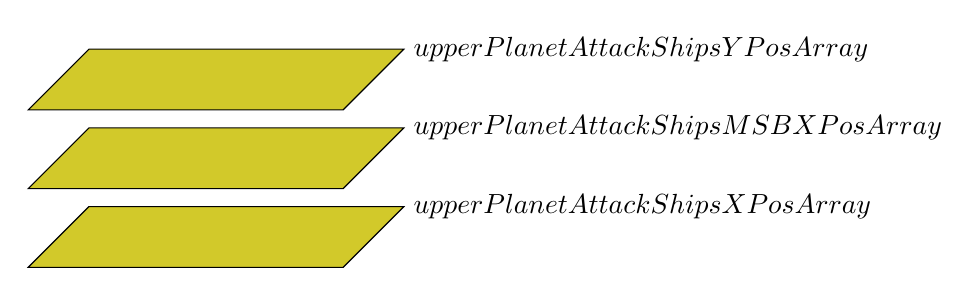
\begin{tikzpicture}
      \draw[fill=yellow!80!black] (0,1,0) -- (4,1,0)--(4,1,2)--(0,1,2)--cycle;
      \node[right] at (4,1,0) {$\icode{upperPlanetAttackShipsXPosArray\index{upperPlanetAttackShipsXPosArray}}$};
      \draw[fill=yellow!80!black] (0,2,0) -- (4,2,0)--(4,2,2)--(0,2,2)--cycle;
      \node[right] at (4,2,0) {$\icode{upperPlanetAttackShipsMSBXPosArray\index{upperPlanetAttackShipsMSBXPosArray}}$};
      \draw[fill=yellow!80!black] (0,3,0) -- (4,3,0)--(4,3,2)--(0,3,2)--cycle;
      \node[right] at (4,3,0) {$\icode{upperPlanetAttackShipsYPosArray\index{upperPlanetAttackShipsYPosArray}}$};
      \end{tikzpicture}
    \end{adjustbox}

  }\caption{The stack after the code above has run with \icode{upperPlanetAttackShipsXPosArray\index{upperPlanetAttackShipsXPosArray}} at the top.}
\end{figure}

With our position data safely stashed away on the stack we now decide which planet\index{planet} we're on:

\begin{lstlisting}[caption= ,escapechar=\%]
        ; Are we on the top or bottom planet%\index{planet}%?
        TXA
        AND #$08
        BNE LowerPlanetAttackShipBehaviour%\index{LowerPlanetAttackShipBehaviour}%
\end{lstlisting}

If we're on the upper planet\index{planet} we use \icode{SetXToIndexOfShipThatNeedsReplacing\index{SetXToIndexOfShipThatNeedsReplacing}} to look in the \icode{activeShipsWaveDataHiPtrArray\index{activeShipsWaveDataHiPtrArray}} for any ships that
need replacing between positions \icode{\$02} and \icode{\$06}. If we don't find one, we return early:

\begin{lstlisting}[escapechar=\%]
        ; We're on the upper planet%\index{planet}%.
        LDX #$02
ProcessAttackShipBehaviour%\index{ProcessAttackShipBehaviour}%   
        JSR SetXToIndexOfShipThatNeedsReplacing%\index{SetXToIndexOfShipThatNeedsReplacing}%
        BEQ ResetAndReturnFromAttackShipBehaviour%\index{ResetAndReturnFromAttackShipBehaviour}%
\end{lstlisting}

If we do find one we can now pull (or 'pop') the positional data we stored away in the stack and assign that to the once-dead
ship. First we use the index we retrieved to \icode{X} to get the ship's index (\icode{Y}) into the positional arrays:

\begin{lstlisting}[escapechar=\%]
        LDY indexIntoUpperPlanetAttackShipXPosAndYPosArray,X
\end{lstlisting}

Then we pop the first positional item \icode{upperPlanetAttackShipsYPosArray\index{upperPlanetAttackShipsYPosArray}} from the top of the stack and store in the new
ship's position in the array:

\begin{lstlisting}[caption="\icode{PLA} remove the top item from the stack and stores it in \icode{A},escapechar=\%]
        PLA
        STA upperPlanetAttackShipsYPosArray%\index{upperPlanetAttackShipsYPosArray}% + $01,Y
\end{lstlisting}

The stack now looks like this, popping from the stack has the effect of removing the first item:

\begin{figure}[H]
  {
    \setlength{\tabcolsep}{3.0pt}
    \setlength\cmidrulewidth{\heavyrulewidth} % Make cmidrule = 
    \begin{adjustbox}{width=10cm,center}
      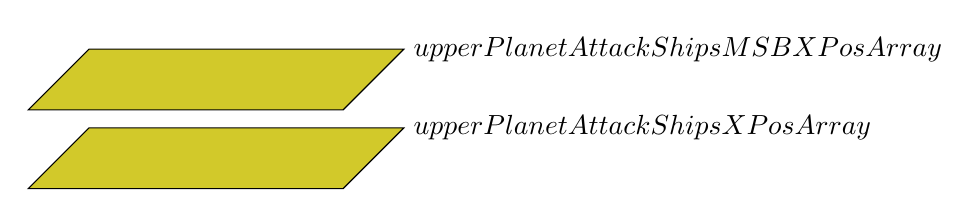
\begin{tikzpicture}
      \draw[fill=yellow!80!black] (0,2,0) -- (4,2,0)--(4,2,2)--(0,2,2)--cycle;
      \node[right] at (4,2,0) {$\icode{upperPlanetAttackShipsXPosArray\index{upperPlanetAttackShipsXPosArray}}$};
      \draw[fill=yellow!80!black] (0,3,0) -- (4,3,0)--(4,3,2)--(0,3,2)--cycle;
      \node[right] at (4,3,0) {$\icode{upperPlanetAttackShipsMSBXPosArray\index{upperPlanetAttackShipsMSBXPosArray}}$};
      \end{tikzpicture}
    \end{adjustbox}

  }
\end{figure}

Then we pop the rest of the items one by one and assign them to the new ship. We ignore the sprite's MXB offset if it is
zero:
\begin{lstlisting}[caption=\icode{PLA} remove the top item from the stack and stores it in \icode{A}.,escapechar=\%]
        PLA
        BEQ MSBXPosOffsetIzZero%\index{MSBXPosOffsetIzZero}%

        LDA attackShipsMSBXPosOffsetArray%\index{attackShipsMSBXPosOffsetArray}% + $01,X
MSBXPosOffsetIzZero%\index{MSBXPosOffsetIzZero}%   
        STA upperPlanetAttackShipsMSBXPosArray%\index{upperPlanetAttackShipsMSBXPosArray}% + $01,Y
        PLA
        STA upperPlanetAttackShipsXPosArray%\index{upperPlanetAttackShipsXPosArray}% + $01,Y
        PLA

        ; Byte 8 of Wave Data gets loaded now. Bytes 8 and 9
        ; contain the hi/lo ptrs to the alternate enemy data.
        LDY #$07
        JMP UpdateWaveDataPointersForCurrentEnemy%\index{UpdateWaveDataPointersForCurrentEnemy}%
\end{lstlisting}

Now that we have set up the positional data for the new enemy we load all its other features from the data pointed
to by Byte 8-9:

\begin{lstlisting}[caption= ,escapechar=\%]
        ; Byte 8 of Wave Data gets loaded now. Bytes 8 and 9
        ; contain the hi/lo ptrs to the alternate enemy data.
        LDY #$07
        JMP UpdateWaveDataPointersForCurrentEnemy%\index{UpdateWaveDataPointersForCurrentEnemy}%
\end{lstlisting}

Let's take a closer look at this routine\index{routine} \icode{UpdateWaveDataPointersForCurrentEnemy\index{UpdateWaveDataPointersForCurrentEnemy}}. What it does in this
instance is take the address pointed to by Bytes 8 and 9 and load the data there using the routine\index{routine}
\icode{GetWaveDataForNewShip\index{GetWaveDataForNewShip}}. To be used in this way the values in Bytes 8 and 9 are combined and treated
as an address in memory. For example if Byte 8 contains \icode{\$70} and Byte 9 contains \icode{\$13} they
are treated as providing the address \icode{\$1370}. This is the location where the enemy data for
\icode{planet1Level8Data\index{planet1Level8Data}} is kept so that is what is loaded.



\begin{figure}[H]
  {
    \setlength{\tabcolsep}{3.0pt}
    \setlength\cmidrulewidth{\heavyrulewidth} % Make cmidrule = 
    \begin{adjustbox}{width=7cm,center}
      \begin{tabular}{rrll}
        \toprule
        Planet &   Level & Byte 6    & Bytes 7-8                   \\
        \midrule
        1 &      11 & \$03       & smallDotWaveData\index{smallDotWaveData}         \\
        1 &      14 & \$03       & planet1Level8Data\index{planet1Level8Data}        \\
        2 &      19 & \$0C       & landGilbyAsEnemy\index{landGilbyAsEnemy}         \\
        3 &       4 & \$04       & gilbyLookingLeft\index{gilbyLookingLeft}         \\
        3 &       6 & \$04       & planet3Level6Additional\index{planet3Level6Additional}  \\
        4 &      19 & \$01       & planet4Level19Additional\index{planet4Level19Additional} \\
        5 &       3 & \$01       & planet5Level3Additional\index{planet5Level3Additional}  \\
        5 &       5 & \$05       & planet5Level5Additional\index{planet5Level5Additional}  \\
        5 &      14 & \$06       & llamaWaveData\index{llamaWaveData}            \\
        \addlinespace
        \bottomrule
        \multicolumn{4}{@{}l@{}}{Byte 6 : Whether a specific attack behaviour is used.}\\
        \multicolumn{4}{@{}l@{}}{Bytes 7-8 : Lo and Hi Ptr for alternate enemy mode}\\
      \end{tabular}

    \end{adjustbox}

  }\caption{Actual use of Bytes 6, 7, and 8. Note that the value in Byte 6 doesn't matter, as long as it's non-zero.}
\end{figure}


\section{Bytes 22-23: The Bytes of Death}
\begin{figure}[H]
  {
    \setlength{\tabcolsep}{3.0pt}
    \setlength\cmidrulewidth{\heavyrulewidth} % Make cmidrule = 
	\centering
	\def\MULTICOLORONE{white}
	\def\MULTICOLORTWO{red}
	\def\SPRITECOLOR{gray}
	\begin{subfigure}{0.3\textwidth}
		\input{sprites/LICKER_SHIP1}
	\end{subfigure}
	\begin{subfigure}{0.3\textwidth}
		\input{sprites/LICKERSHIP2}
	\end{subfigure}
	\begin{subfigure}{0.3\textwidth}
		\input{sprites/LICKERSHIP3}
	\end{subfigure}
  }\caption[position=top]{These arseholes.}
\end{figure}

An irritating early hurdle in Iridis Alpha's gameplay is the behaviour of the lickerships in the game's third level.
When shot the enemies\index{enemies} turn into lickerships that seek out the player and then stick to them, sapping the player's energy\index{energy}
until they lose a life. This behaviour is defined by Bytes 22 and 23. 

\begin{lstlisting}[escapechar=\%]
lickerShipWaveData%\index{lickerShipWaveData}% = $1118
  ..
  ; Byte 22 (Index $16): Stickiness%\index{Stickiness}% factor, does the enemy stick to
  ; the player sapping their energy%\index{energy}% if they're near them?
  .BYTE $01
  ; Byte 23 (Index $17): Does the enemy gravitate quickly toward the
  ; player when its been shot? (Typical lickership%\index{lickership}% behaviour)
  .BYTE $01
  ..
\end{lstlisting}

Implementing each of these is relatively straighforward. Since the gilby is always in the centre of the screen\index{screen} (on the
X axis at least), all an enemy has to do is figure out whether the gilby is above or below it and move in that direction.
If we leave out the slightly complicated logic to figure out where the gilby is relative to us, we are left with this:

\begin{lstlisting}[escapechar=\%]
MaybeQuicklyGravitatesToGilby%\index{MaybeQuicklyGravitatesToGilby}%
  ; Byte 23:  Does the enemy gravitate quickly towards the gilby
  ; when it is shot?
  LDY #$17
  LDA (currentShipWaveDataLoPtr%\index{currentShipWaveDataLoPtr}%),Y
  BEQ MaybeStickyAttackShipBehaviour%\index{MaybeStickyAttackShipBehaviour}%
  ...
  ; Figure out the relative position of the gilby and
  ; store it in positionRelativeToGilby%\index{positionRelativeToGilby}%
  ...
  ; Now decide whether to move up or down.
  CMP positionRelativeToGilby%\index{positionRelativeToGilby}%
  BEQ NoVerticalMovementRequired%\index{NoVerticalMovementRequired}%
  BMI MoveDownToGilby%\index{MoveDownToGilby}%
MoveUpToGilby%\index{MoveUpToGilby}%
  DEC yPosMovementForUpperPlanetAttackShips%\index{yPosMovementForUpperPlanetAttackShips}%,X
  DEC yPosMovementForUpperPlanetAttackShips%\index{yPosMovementForUpperPlanetAttackShips}%,X
MoveDownToGilby%\index{MoveDownToGilby}%
  INC yPosMovementForUpperPlanetAttackShips%\index{yPosMovementForUpperPlanetAttackShips}%,X
NoVerticalMovementRequired%\index{NoVerticalMovementRequired}%
  LDA indexForActiveShipsWaveData%\index{indexForActiveShipsWaveData}%,X
  TAX
\end{lstlisting}

Sticking to the gilby involves the same logic but along the horizontal axis. After all if we're sticking to the gilby
we want to stay in the centre of the screen\index{screen}.

\begin{lstlisting}[escapechar=\%]
MaybeStickyAttackShipBehaviour%\index{MaybeStickyAttackShipBehaviour}%   
  ; Byte 22: Does the enemy have the stickiness%\index{stickiness}% behaviour?
  LDY #$16
  LDA (currentShipWaveDataLoPtr%\index{currentShipWaveDataLoPtr}%),Y
  BEQ MaybeSwitchToAlternateEnemyPattern%\index{MaybeSwitchToAlternateEnemyPattern}%
  ...
  ; Figure out the relative position of the gilby and
  ; store it in positionRelativeToGilby%\index{positionRelativeToGilby}%
  ...
  CMP positionRelativeToGilby%\index{positionRelativeToGilby}%
  BMI MoveRightToGilby%\index{MoveRightToGilby}%
MoveLeftToGilby%\index{MoveLeftToGilby}%   
  DEC xPosMovementForUpperPlanetAttackShip%\index{xPosMovementForUpperPlanetAttackShip}%,X
  DEC xPosMovementForUpperPlanetAttackShip%\index{xPosMovementForUpperPlanetAttackShip}%,X
MoveRightToGilby%\index{MoveRightToGilby}%   
  INC xPosMovementForUpperPlanetAttackShip%\index{xPosMovementForUpperPlanetAttackShip}%,X
NoHorizontalMovementRequired%\index{NoHorizontalMovementRequired}%   
  LDA indexForActiveShipsWaveData%\index{indexForActiveShipsWaveData}%,X
  TAX
\end{lstlisting}

\section{Byte 35: Energy Multiplier}
When an enemy is struck this byte contains the multiplier applied to the player's energy\index{energy} boost:

\begin{lstlisting}[escapechar=\%]
IncreaseEnergyTopOnly%\index{IncreaseEnergyTopOnly}%
    LDY #$23
    LDA (currentShipWaveDataLoPtr%\index{currentShipWaveDataLoPtr}%),Y
    BEQ NormalTopEnergyIncrease%\index{NormalTopEnergyIncrease}%
    STA energyChangeCounter%\index{energyChangeCounter}%
EnergyTopIncreaseLoop%\index{EnergyTopIncreaseLoop}%
    JSR IncreaseEnergyTop%\index{IncreaseEnergyTop}%
    DEC energyChangeCounter%\index{energyChangeCounter}%
    BNE EnergyTopIncreaseLoop%\index{EnergyTopIncreaseLoop}%
    RTS

NormalTopEnergyIncrease%\index{NormalTopEnergyIncrease}%
    JMP IncreaseEnergyTop%\index{IncreaseEnergyTop}%
    ;Returns%\index{Returns}%
\end{lstlisting}

The above is for the top planet\index{planet} energy\index{energy} counter, the logic for the bottom planet\index{planet} is identical:

\begin{lstlisting}[escapechar=\%]
IncreaseEnergyBottomOnly%\index{IncreaseEnergyBottomOnly}%
    LDY #$23
    LDA (currentShipWaveDataLoPtr%\index{currentShipWaveDataLoPtr}%),Y
    BEQ NormalBottomEnergyIncrease%\index{NormalBottomEnergyIncrease}%
    STA energyChangeCounter%\index{energyChangeCounter}%
EnergyBottomIncreaseLoop%\index{EnergyBottomIncreaseLoop}%
    JSR IncreaseEnergyBottom%\index{IncreaseEnergyBottom}%
    DEC energyChangeCounter%\index{energyChangeCounter}%
    BNE EnergyBottomIncreaseLoop%\index{EnergyBottomIncreaseLoop}%
    RTS

NormalBottomEnergyIncrease%\index{NormalBottomEnergyIncrease}%
    JMP IncreaseEnergyBottom%\index{IncreaseEnergyBottom}%
    ;Returns%\index{Returns}%
\end{lstlisting}

\subfile{titlescreen/energy_tilesheet}

Actually writing the updated energy\index{energy} level to the screen\index{screen} uses the tileset above in the routine\index{routine}
\icode{IncreaseEnergyTop\index{IncreaseEnergyTop}}:
\begin{lstlisting}[escapechar=\%]
IncreaseEnergyTop%\index{IncreaseEnergyTop}%
    STX temporaryStorageForXRegister%\index{temporaryStorageForXRegister}%
    LDX currEnergyTop%\index{currEnergyTop}%
    DEC SCREEN_RAM%\index{SCREEN\_RAM}% + LINE22_COL3%\index{LINE22\_COL3}%,X
    LDA SCREEN_RAM%\index{SCREEN\_RAM}% + LINE22_COL3%\index{LINE22\_COL3}%,X
    CMP #$7F
    BNE b547B
    ; Note the reference to the index $80 of the first tile
    ; in the set above.
    LDA #$80 
    STA SCREEN_RAM%\index{SCREEN\_RAM}% + LINE22_COL3%\index{LINE22\_COL3}%,X
    INX
    STX currEnergyTop%\index{currEnergyTop}%
    CPX #$08
    BEQ GilbyDiesFromExcessEnergy%\index{GilbyDiesFromExcessEnergy}%
    LDA #$87
    STA SCREEN_RAM%\index{SCREEN\_RAM}% + LINE22_COL3%\index{LINE22\_COL3}%,X
    BNE b547B
\end{lstlisting}

Byte 35 also determines the multiplier applied to the energy\index{energy} sapped from the player in the 
event of a collision with the enemy:

\begin{lstlisting}[escapechar=\%]
UpdateEnergyLevelsAfterCollision%\index{UpdateEnergyLevelsAfterCollision}%
    ; Check if the enemy saps energy%\index{energy}% from the gilby?
    LDY #$23
    LDA (currentShipWaveDataLoPtr%\index{currentShipWaveDataLoPtr}%),Y
    BEQ LoadExplosionData

    LDA #<shipCollidedWithGilbySound%\index{shipCollidedWithGilbySound}%
    STA primarySoundEffectLoPtr%\index{primarySoundEffectLoPtr}%
    LDA #>shipCollidedWithGilbySound%\index{shipCollidedWithGilbySound}%
    STA primarySoundEffectHiPtr%\index{primarySoundEffectHiPtr}%
    JSR ResetRepetitionForPrimarySoundEffect%\index{ResetRepetitionForPrimarySoundEffect}%
    LDA #$0E
    STA gilbyExploding%\index{gilbyExploding}%
    LDA #$02
    STA starFieldInitialStateArray%\index{starFieldInitialStateArray}% - $01
    LDA currentGilbySpeed%\index{currentGilbySpeed}%
    EOR #$FF
    CLC
    ADC #$01
    STA currentGilbySpeed%\index{currentGilbySpeed}%

    LDA setToZeroIfOnUpperPlanet%\index{setToZeroIfOnUpperPlanet}%
    BEQ EnergyUpdateTopPlanet%\index{EnergyUpdateTopPlanet}%

    LDA extraAmountToDecreaseEnergyByBottomPlanet%\index{extraAmountToDecreaseEnergyByBottomPlanet}%
    BNE LoadExplosionData
    ; Y is still $23.
    LDA (currentShipWaveDataLoPtr%\index{currentShipWaveDataLoPtr}%),Y
    JSR AugmentAmountToDecreaseEnergyByBountiesEarned
    STA extraAmountToDecreaseEnergyByBottomPlanet%\index{extraAmountToDecreaseEnergyByBottomPlanet}%
    BNE LoadExplosionData

EnergyUpdateTopPlanet%\index{EnergyUpdateTopPlanet}%   
    LDA extraAmountToDecreaseEnergyByTopPlanet%\index{extraAmountToDecreaseEnergyByTopPlanet}%
    BNE LoadExplosionData
    ; Y is still $23.
    LDA (currentShipWaveDataLoPtr%\index{currentShipWaveDataLoPtr}%),Y
    JSR AugmentAmountToDecreaseEnergyByBountiesEarned
    STA extraAmountToDecreaseEnergyByTopPlanet%\index{extraAmountToDecreaseEnergyByTopPlanet}%
LoadExplosionData
    LDY #$1E
    JMP UpdateWaveDataPointersForCurrentEnemy%\index{UpdateWaveDataPointersForCurrentEnemy}%
    ; Returns%\index{Returns}%

\end{lstlisting}

\section{Byte 34: Score for Hitting the Enemy}
This is used to augment the score received for hitting the enemy.
\begin{lstlisting}[escapechar=\%]
    ; Get the points for hitting enemies%\index{enemies}% in this level
    ; from the wave data.
AddPointsForHittingEnemy%\index{AddPointsForHittingEnemy}%   
    ; Byte 34
    LDY #$22
    LDA (currentShipWaveDataLoPtr%\index{currentShipWaveDataLoPtr}%),Y
    ..
    ADC pointsEarnedTopPlanetByte1%\index{pointsEarnedTopPlanetByte1}%
    STA pointsEarnedTopPlanetByte1%\index{pointsEarnedTopPlanetByte1}%
\end{lstlisting}

\section{Bytes 9-11: A Clever Plan}
\begin{figure}[H]
  {
    \setlength{\tabcolsep}{3.0pt}
    \setlength\cmidrulewidth{\heavyrulewidth} % Make cmidrule = 
    \begin{adjustbox}{width=10cm, center}

      \begin{tabular}{lll}
        \toprule
        Byte    & Value                     & Description                                                        \\
        \midrule
        Byte 9  & nullPtr\index{nullPtr}                   & \textbf{Unused} Lo Ptr to an arbitrary run of Bytes 18-21.\\
        Byte 10 & nullPtr\index{nullPtr}                   & \textbf{Unused} Hi Ptr to an arbitrary run of Bytes 18-21.\\
        Byte 11 & \$00                       & \textbf{Unused} Rate limiter for use of Bytes 9 and 10. \\
        .. & ..                       & ..\\
        Byte 18 & \$06                       & X Pos movement\index{movement} for attack ship.                                    \\
        Byte 19 & \$01                       & Y Pos movement\index{movement} pattern\index{pattern} for attack ship.                            \\
        Byte 20 & \$01                       & X Pos Frame Rate for Attack ship.                                  \\
        Byte 21 & \$01                       & Y Pos Frame Rate for Attack ship.                                  \\
        \bottomrule
      \end{tabular}
    \end{adjustbox}
  }\caption{Bytes 9 to 11, and 18 to 21.}
\end{figure}
Bytes 9 to 11 were intended to carry out a clever plan that was probably too clever for its own
good and as a result ended up being dropped. The idea was that Bytes 9 and 10 would point to 
Bytes 18 to 21 in another set of level data, enabling the enemy to have a second phase of movement\index{movement}
behaviour in addition to its native movement\index{movement}.

The routine\index{routine} for processing these bytes appears in \icode{UpdateAttackShipDataForNewShip\index{UpdateAttackShipDataForNewShip}}. 

\begin{lstlisting}[escapechar=\%]
UpdateAttackShipDataForNewShip%\index{UpdateAttackShipDataForNewShip}%

  ; Byte 10:
  LDY #10
  LDA (currentShipWaveDataLoPtr%\index{currentShipWaveDataLoPtr}%),Y
  BEQ MaybeQuicklyGravitatesToGilby%\index{MaybeQuicklyGravitatesToGilby}%

UnusedRoutine%\index{UnusedRoutine}%
  ; As above, this section is never reached because Byte 10
  ; is never set.
  DEC someKindOfRateLimitingForAttackWaves%\index{someKindOfRateLimitingForAttackWaves}%,X
  BNE MaybeQuicklyGravitatesToGilby%\index{MaybeQuicklyGravitatesToGilby}%

  ; Store Bytes 10 and 11 in newMovementLoPtr%\index{newMovementLoPtr}% and 
  ; newMovementHiPtr%\index{newMovementHiPtr}% respectively.
  STA newMovementHiPtr%\index{newMovementHiPtr}%
  DEY
  ; Byte 9: Y is now $09.
  LDA (currentShipWaveDataLoPtr%\index{currentShipWaveDataLoPtr}%),Y
  STA newMovementLoPtr%\index{newMovementLoPtr}%

  ; Byte 11 in the wave data defines some kind of rate limiting%\index{limiting}%.
  LDY #11
  LDA (currentShipWaveDataLoPtr%\index{currentShipWaveDataLoPtr}%),Y
  STA someKindOfRateLimitingForAttackWaves%\index{someKindOfRateLimitingForAttackWaves}%,X

  ; newMovementLoPtr%\index{newMovementLoPtr}% would have pointed to some section of Bytes 18-21
  ; in another set of leval data. So it would get loaded here to
  ; populate the behaviour for the attack wave.
  LDY indexForYPosMovementForUpperPlanetAttackShips,X
  LDA orderForUpdatingPositionOfAttackShips%\index{orderForUpdatingPositionOfAttackShips}%,X
  TAX
  LDA (newMovementLoPtr%\index{newMovementLoPtr}%),Y
  CMP #$80
  BEQ SkipLoadingWaveData%\index{SkipLoadingWaveData}%

  ; Load Byte 18, the X Pos movememnt%\index{movememnt}%.
  LDA (newMovementLoPtr%\index{newMovementLoPtr}%),Y
  STA xPosMovementForUpperPlanetAttackShip%\index{xPosMovementForUpperPlanetAttackShip}%,X
  
  ; Load Byte 19, the Y Pos movement%\index{movement}%.
  INY
  LDA (newMovementLoPtr%\index{newMovementLoPtr}%),Y
  STA yPosMovementForUpperPlanetAttackShips%\index{yPosMovementForUpperPlanetAttackShips}%,X

  ; Load Byte 20, the X Pos framerate%\index{framerate}%.
  INY
  LDA (newMovementLoPtr%\index{newMovementLoPtr}%),Y
  STA upperPlanetInitialXPosFrameRateForAttackShip%\index{upperPlanetInitialXPosFrameRateForAttackShip}%,X
  STA upperPlanetXPosFrameRateForAttackShip%\index{upperPlanetXPosFrameRateForAttackShip}%,X

  ; Load Byte 21, the Y Pos framerate%\index{framerate}%.
  INY
  LDA (newMovementLoPtr%\index{newMovementLoPtr}%),Y
  STA upperPlanetInitialYPosFrameRateForAttackShips,X
  STA upperPlanetYPosFrameRateForAttackShips%\index{upperPlanetYPosFrameRateForAttackShips}%,X

  INY
  LDA indexForActiveShipsWaveData%\index{indexForActiveShipsWaveData}%,X
  TAX
  TYA
  STA indexForYPosMovementForUpperPlanetAttackShips,X
  JMP MaybeQuicklyGravitatesToGilby%\index{MaybeQuicklyGravitatesToGilby}%
\end{lstlisting}

Since Bytes 9 to 11 are zero in all level data, the routine\index{routine} is never run. On balance the idea does seem
unnecessarily complex: why not just load a completely new set of level data with modified behaviour and
the same sprite? This uses up more space overall but it is certainly easier to manage. Indeed, much
of the level data is given over to chaining level data in this way. Let's look at that now.


\section{Bytes 15-17: Sprite Switching}
Byte 15 defines a value that is periodically decremented and when it reaches zero the level data pointed
to by Bytes 16 and 17 is loaded. This is used in the very first level to switch the main sprite colour
of the flying UFOs. 

\begin{figure}[H]

  {
    \setlength{\tabcolsep}{3.0pt}
    \setlength\cmidrulewidth{\heavyrulewidth} % Make cmidrule = 
    \begin{adjustbox}{width=13cm}

      \begin{tabular}{lll}
        \toprule
        Byte    & Value                     & Description                                                        \\
        \midrule
Byte 15 & \$40                       & Update rate for periodically switching to wave defined in Bytes 16-17. \\
 Byte 16 & planet1Level1Data2ndStage\index{planet1Level1Data2ndStage} & Lo Ptr to the wave data we switch to periodically.               \\
 Byte 17 & planet1Level1Data2ndStage\index{planet1Level1Data2ndStage} & Hi Ptr to the wave data we switch to periodically.               \\
        \bottomrule
      \end{tabular}
    \end{adjustbox}
  }\caption{\icode{planet1Level1Data\index{planet1Level1Data}}: Bytes 15 to 17 for Level 1 on the Sheep Planet.}
\end{figure}

The way it works is Byte 15 is loaded to the appropriate position in \icode{updateRateForAttack\-Ships\index{updateRateForAttackShips}}:

\begin{lstlisting}[escapechar=\%]
GetWaveDataForNewShip%\index{GetWaveDataForNewShip}%
  ..
  ; Byte 15; Update Rate for Attack Waves
  LDY #15
  LDA (currentShipWaveDataLoPtr%\index{currentShipWaveDataLoPtr}%),Y
  STA updateRateForAttackShips%\index{updateRateForAttackShips}%,X
\end{lstlisting}

This is then periodically decremented in \icode{GetNewShipDataFromDataStore\index{GetNewShipDataFromDataStore}}. When it reaches zero we 
end up jumping\index{jumping} to \icode{SwitchToAlternatingWaveData\index{SwitchToAlternatingWaveData}}:
\begin{lstlisting}[escapechar=\%]
  DEC updateRateForAttackShips%\index{updateRateForAttackShips}%,X
  BNE UpdateAttackShipDataForNewShip%\index{UpdateAttackShipDataForNewShip}%
  ; Byte 14: Controls the rate at which new enemies%\index{enemies}% are added.
  ; This is only set when the current ship data is defaultExplosion%\index{defaultExplosion}%
  ; so in most cases we will go straight to SwitchToAlternatingWaveData%\index{SwitchToAlternatingWaveData}%.
  LDY #14
  LDA (currentShipWaveDataLoPtr%\index{currentShipWaveDataLoPtr}%),Y
  BEQ SwitchToAlternatingWaveData%\index{SwitchToAlternatingWaveData}%
\end{lstlisting}

This now pulls in Bytes 16 and 17 from the level data and uses them as the address of the level data to 
switch to:
\begin{lstlisting}[escapechar=\%]
SwitchToAlternatingWaveData%\index{SwitchToAlternatingWaveData}%   
  LDY #16

;-------------------------------------------------------
; UpdateWaveDataPointersForCurrentEnemy%\index{UpdateWaveDataPointersForCurrentEnemy}%
;-------------------------------------------------------
UpdateWaveDataPointersForCurrentEnemy%\index{UpdateWaveDataPointersForCurrentEnemy}%
  ; Byte 16  Y has been set to 16 above, so we're pulling in the pointer%\index{pointer}%
  ; to the second tranche of wave data for this level. 
  ; Or Y has been set by the caller.
  LDA (currentShipWaveDataLoPtr%\index{currentShipWaveDataLoPtr}%),Y
  PHA
  INY
  ; Byte 17
  LDA (currentShipWaveDataLoPtr%\index{currentShipWaveDataLoPtr}%),Y

  ; If we have a nullPtr%\index{nullPtr}% then there's no wave data to get
  ; so the enemy ship can be cleared out and we can return.
  BEQ ClearDeadShipFromLevelData%\index{ClearDeadShipFromLevelData}%

  STA activeShipsWaveDataHiPtrArray%\index{activeShipsWaveDataHiPtrArray}%,X
  STA currentShipWaveDataHiPtr%\index{currentShipWaveDataHiPtr}%
  PLA
  STA currentShipWaveDataLoPtr%\index{currentShipWaveDataLoPtr}%
  STA activeShipsWaveDataLoPtrArray%\index{activeShipsWaveDataLoPtrArray}%,X
\end{lstlisting}

In the case of Level 1 this second set of wave data is at \icode{planet1Level1Data2ndStage\index{planet1Level1Data2ndStage}}. This data is more
or less the same as \icode{planet1Level1Data\index{planet1Level1Data}} with the exception of the bytes in the table below.

\begin{figure}[H]

  {
    \setlength{\tabcolsep}{3.0pt}
    \setlength\cmidrulewidth{\heavyrulewidth} % Make cmidrule = 
    \begin{adjustbox}{width=13cm}

      \begin{tabular}{lll}
        \toprule
        Byte    & Value                     & Description                                                        \\
        \midrule
  Byte 0  & \icode{\$11}                       & Index into array for sprite colour                                  \\
 Byte 16 & planet1Level1Data\index{planet1Level1Data} & Lo Ptr to the wave data we switch to periodically.               \\
 Byte 17 & planet1Level1Data\index{planet1Level1Data} & Hi Ptr to the wave data we switch to periodically.               \\
        \bottomrule
      \end{tabular}
    \end{adjustbox}
  }\caption{\icode{planet1Level1Data\index{planet1Level1Data}}: Bytes 15 to 17 for Level 1 on the Sheep Planet.}
\end{figure}

The effect therefore is that the main sprite colour changes (although the sprite stays the same) and when the 
periodic decrementing of Byte 15 reaches zero again it will switch back to \icode{planet1Level1Data\index{planet1Level1Data}}. This 
switching back and forth will continue for as long as the enemy does not collide with anything or is not hit.

\begin{figure}[H]
  {
    \setlength{\tabcolsep}{3.0pt}
    \setlength\cmidrulewidth{\heavyrulewidth} % Make cmidrule = 
	\centering
	\def\MULTICOLORONE{white}
	\def\MULTICOLORTWO{red}
	\def\SPRITECOLOR{blue}
	\begin{subfigure}{0.3\textwidth}
		\input{sprites/FLYING_SAUCER1}
	\end{subfigure}
	\begin{subfigure}{0.3\textwidth}
		\input{sprites/FLYING_SAUCER2}
	\end{subfigure}
	\begin{subfigure}{0.3\textwidth}
		\input{sprites/FLYING_SAUCER3}
	\end{subfigure}
}\caption[position=top]{Level 1 Sprite as given by \icode{level1Planet1Data}.}
\end{figure}

\begin{figure}[H]
  {
    \setlength{\tabcolsep}{3.0pt}
    \setlength\cmidrulewidth{\heavyrulewidth} % Make cmidrule = 
	\centering
	\def\MULTICOLORONE{white}
	\def\MULTICOLORTWO{red}
	\def\SPRITECOLOR{c64_purple}
	\begin{subfigure}{0.3\textwidth}
		\input{sprites/FLYING_SAUCER1}
	\end{subfigure}
	\begin{subfigure}{0.3\textwidth}
		\input{sprites/FLYING_SAUCER2}
	\end{subfigure}
	\begin{subfigure}{0.3\textwidth}
		\input{sprites/FLYING_SAUCER3}
	\end{subfigure}
}\caption[position=top]{Level 1 Sprite as given by \icode{level1Planet1Data2ndStage}.}
\end{figure}

\section{Bytes 28-29: Data to Load When Hit by a Bullet}
\begin{figure}[H]

  {
    \setlength{\tabcolsep}{3.0pt}
    \setlength\cmidrulewidth{\heavyrulewidth} % Make cmidrule = 
    \begin{adjustbox}{width=10cm,center}

      \begin{tabular}{lll}
        \toprule
        Byte    & Value                     & Description                                                        \\
        \midrule
 Byte 28 & spinningRings\index{spinningRings}             & Lo Ptr for data to switch to when hit by bullet.                                    \\
 Byte 29 & spinningRings\index{spinningRings}             & Hi Ptr for data to switch to when hit by bullet.                                    \\
        \bottomrule
      \end{tabular}
    \end{adjustbox}
  }\caption{\icode{planet1Level1Data\index{planet1Level1Data}}: Bytes 28 to 29 for Level 1 on the Sheep Planet.}
\end{figure}

Bytes 28 and 29 define the level data to load when struck by a bullet. In the case of our
flying UFOs this is the spinning\index{spinning} rings.

\begin{figure}[H]
  {
    \setlength{\tabcolsep}{1.0pt}
    \setlength\cmidrulewidth{\heavyrulewidth} % Make cmidrule = 
	\centering
	\def\MULTICOLORONE{white}
	\def\MULTICOLORTWO{yellow}
	\def\SPRITECOLOR{yellow}
	\begin{subfigure}{0.23\textwidth}
		\input{sprites/SPINNING_RING1}
	\end{subfigure}
	\begin{subfigure}{0.23\textwidth}
		\input{sprites/SPINNING_RING2}
	\end{subfigure}
	\begin{subfigure}{0.23\textwidth}
		\input{sprites/SPINNING_RING3}
	\end{subfigure}
	\begin{subfigure}{0.23\textwidth}
		\input{sprites/SPINNING_RING4}
	\end{subfigure}
  }\caption[position=top]{The sprites\index{sprites} used to animate the spinning\index{spinning} rings.}
\end{figure}

\begin{lstlisting}[escapechar=\%]
UpdateScoresAfterHittingShipWithBullet%\index{UpdateScoresAfterHittingShipWithBullet}%
    ..
    ; Byte 29: Load the explosion%\index{explosion}% animation%\index{animation}%, if there is one. For most
    ; enemies%\index{enemies}% this is the spinning%\index{spinning}% rings defined by spinningRings%\index{spinningRings}%.
LoadExplosionAnimation%\index{LoadExplosionAnimation}%   
    LDY #29
    LDA (currentShipWaveDataLoPtr%\index{currentShipWaveDataLoPtr}%),Y
    BEQ CheckForCollisionsBeforeUpdatingCurrentShipsWaveData
    ; There's a Hi Ptr for the explosion%\index{explosion}% animation%\index{animation}%, so decrement
    ; Y to point it at the Lo Ptr and load the ptrs as the new
    ; wave data for the enemy.
    DEY
    JMP UpdateWaveDataPointersForCurrentEnemy%\index{UpdateWaveDataPointersForCurrentEnemy}%
    ;Returns%\index{Returns}%
\end{lstlisting}

This is also the path used to load the licker ships after the relatively inoffensive flying blue dots have
been struck by a bullet.

\begin{figure}[H]
  {
  \setlength{\tabcolsep}{3.0pt}
  \setlength\cmidrulewidth{\heavyrulewidth} % Make cmidrule = 
  \begin{adjustbox}{width=12cm}

\begin{tabular}{lll}
\toprule
 Byte    & Value                     & Description                                                        \\
\midrule
 Byte 0  & \$05                       & Index into array for sprite colour                                  \\
 Byte 1  & FLYING\_DOT1               & Sprite value for the attack ship on the upper planet\index{planet}               \\
 Byte 28 & lickerShipWaveData\index{lickerShipWaveData}         & Lo Ptr for data to switch to when hit by bullet.                                    \\
 Byte 29 & lickerShipWaveData\index{lickerShipWaveData}         & Hi Ptr for data to switch to when hit by bullet.                                    \\
\bottomrule
\end{tabular}

  \end{adjustbox}

  }\caption{Sheep Planet - Level 3
.}
\end{figure}

\section{Bytes 30-31: Data to Load After Colliding with the Player}
\begin{figure}[H]

  {
    \setlength{\tabcolsep}{3.0pt}
    \setlength\cmidrulewidth{\heavyrulewidth} % Make cmidrule = 
    \begin{adjustbox}{width=13cm}

      \begin{tabular}{lll}
        \toprule
        Byte    & Value                     & Description                                                        \\
        \midrule
 Byte 30 & defaultExplosion\index{defaultExplosion}          & Lo Ptr for data to switch to after colliding\index{colliding} with gilby.                \\
 Byte 31 & defaultExplosion\index{defaultExplosion}          & Hi Ptr for data to switch to after colliding\index{colliding} with gilby.                \\
        \bottomrule
      \end{tabular}
    \end{adjustbox}
  }\caption{\icode{planet1Level1Data\index{planet1Level1Data}}: Bytes 30 to 31 for Level 1 on the Sheep Planet.}
\end{figure}

Bytes 30 and 31 define the level data to load when the enemy has collided with the player. In the case of our
flying UFOs this is the default explosion\index{explosion} animation\index{animation}.

\begin{figure}[H]
  {
    \setlength{\tabcolsep}{3.0pt}
    \setlength\cmidrulewidth{\heavyrulewidth} % Make cmidrule = 
	\centering
	\def\MULTICOLORONE{white}
	\def\MULTICOLORTWO{red}
	\def\SPRITECOLOR{c64_darkgray}
	\begin{subfigure}{0.3\textwidth}
		\input{sprites/EXPLOSION_START}
	\end{subfigure}
	\begin{subfigure}{0.3\textwidth}
		\input{sprites/EXPLOSION_MIDDLE}
	\end{subfigure}
	\begin{subfigure}{0.3\textwidth}
		\input{sprites/EXPLOSION_END}
	\end{subfigure}
  }\caption[position=top]{The sprites\index{sprites} used to animate the collision explosion\index{explosion}.}
\end{figure}

These bytes are only inspected when responding to a collision. The routine\index{routine} \icode{Update\-EnergyLevelsAfterCollision}
first establishes if the enemy saps energy\index{energy} from the gilby by inspecting Byte 35. Once the updated player energy\index{energy}
is calculated the collision explosion\index{explosion} data is loaded.

\begin{lstlisting}[escapechar=\%]
UpdateEnergyLevelsAfterCollision%\index{UpdateEnergyLevelsAfterCollision}%
    ; Byte 35: Check if the enemy saps energy%\index{energy}% from the gilby?
    LDY #35
    LDA (currentShipWaveDataLoPtr%\index{currentShipWaveDataLoPtr}%),Y
    BEQ LoadExplosionData

    LDA #<shipCollidedWithGilbySound%\index{shipCollidedWithGilbySound}%
    STA primarySoundEffectLoPtr%\index{primarySoundEffectLoPtr}%
    LDA #>shipCollidedWithGilbySound%\index{shipCollidedWithGilbySound}%
    STA primarySoundEffectHiPtr%\index{primarySoundEffectHiPtr}%
    JSR ResetRepetitionForPrimarySoundEffect%\index{ResetRepetitionForPrimarySoundEffect}%
    LDA #$0E
    STA gilbyExploding%\index{gilbyExploding}%
    LDA #$02
    STA starFieldInitialStateArray%\index{starFieldInitialStateArray}% - $01
    LDA currentGilbySpeed%\index{currentGilbySpeed}%
    EOR #$FF
    CLC
    ADC #$01
    STA currentGilbySpeed%\index{currentGilbySpeed}%

    LDA setToZeroIfOnUpperPlanet%\index{setToZeroIfOnUpperPlanet}%
    BEQ EnergyUpdateTopPlanet%\index{EnergyUpdateTopPlanet}%

    LDA extraAmountToDecreaseEnergyByBottomPlanet%\index{extraAmountToDecreaseEnergyByBottomPlanet}%
    BNE LoadExplosionData
    ; Y is still 35.
    LDA (currentShipWaveDataLoPtr%\index{currentShipWaveDataLoPtr}%),Y
    JSR AugmentAmountToDecreaseEnergyByBountiesEarned
    STA extraAmountToDecreaseEnergyByBottomPlanet%\index{extraAmountToDecreaseEnergyByBottomPlanet}%
    BNE LoadExplosionData

EnergyUpdateTopPlanet%\index{EnergyUpdateTopPlanet}%   
    LDA extraAmountToDecreaseEnergyByTopPlanet%\index{extraAmountToDecreaseEnergyByTopPlanet}%
    BNE LoadExplosionData
    ; Y is still 35.
    LDA (currentShipWaveDataLoPtr%\index{currentShipWaveDataLoPtr}%),Y
    JSR AugmentAmountToDecreaseEnergyByBountiesEarned
    STA extraAmountToDecreaseEnergyByTopPlanet%\index{extraAmountToDecreaseEnergyByTopPlanet}%

LoadExplosionData
    ; Byte 30: Hi/Lo Ptr for the collision explosion%\index{explosion}% level data.
    LDY #30
    JMP UpdateWaveDataPointersForCurrentEnemy%\index{UpdateWaveDataPointersForCurrentEnemy}%
    ; Returns%\index{Returns}%
\end{lstlisting}

\section{Bytes 24-27 and 32-33: Enemy Phases}
Rather than exploding when first hit, some enemy waves are configured to metamorphose into something else, so they 
end up requiring multiple hits before they oblige the player by finally exploding.

The level data accomodates up to four incarnations in total for an enemy wave.

\begin{figure}[H]

  {
    \setlength{\tabcolsep}{3.0pt}
    \setlength\cmidrulewidth{\heavyrulewidth} % Make cmidrule = 
    \begin{adjustbox}{width=13cm}

      \begin{tabular}{lll}
        \toprule
        Byte    & Value                     & Description                                                        \\
        \midrule
 Byte 24-25 & nullPtr\index{nullPtr}                   & Pointer for second wave of attack ships.                            \\
 Byte 26-27 & nullPtr\index{nullPtr}                   & Pointer for third wave of attack ships.                             \\
 Byte 32-33 & nullPtr                       & Pointer for fourth wave of attack ships.                            \\
        \bottomrule
      \end{tabular}
    \end{adjustbox}
  }\caption{Mostly unused: the contents of these bytes for most levels in the game.}
\end{figure}

\begin{lstlisting}[escapechar=\%]
GetNewShipDataFromDataStore%\index{GetNewShipDataFromDataStore}%
    LDA hasReachedSecondWaveAttackShips%\index{hasReachedSecondWaveAttackShips}%,X
    BEQ No2ndWaveData%\index{No2ndWaveData}%

    LDA #$00
    STA hasReachedSecondWaveAttackShips%\index{hasReachedSecondWaveAttackShips}%,X

    ; Byte 25: The 2nd stage of wave data for this enemy.
    LDY #25
    LDA (currentShipWaveDataLoPtr%\index{currentShipWaveDataLoPtr}%),Y
    BEQ No2ndWaveData%\index{No2ndWaveData}%

    DEY
    JMP UpdateWaveDataPointersForCurrentEnemy%\index{UpdateWaveDataPointersForCurrentEnemy}%

No2ndWaveData%\index{No2ndWaveData}%   
    LDA hasReachedThirdWaveAttackShips%\index{hasReachedThirdWaveAttackShips}%,X
    BEQ No3rdWaveData%\index{No3rdWaveData}%

    LDA #$00
    STA hasReachedThirdWaveAttackShips%\index{hasReachedThirdWaveAttackShips}%,X

    ; Byte 27: The 3rd stage of wave data for this enemy.
    LDY #27
    LDA (currentShipWaveDataLoPtr%\index{currentShipWaveDataLoPtr}%),Y
    BEQ No3rdWaveData%\index{No3rdWaveData}%

    DEY
    JMP UpdateWaveDataPointersForCurrentEnemy%\index{UpdateWaveDataPointersForCurrentEnemy}%

No3rdWaveData%\index{No3rdWaveData}%   
    LDA joystickInput%\index{joystickInput}%
    AND #$10
    BNE No4thWaveData%\index{No4thWaveData}%

    ; Fire is pressed.
    ; Byte 33: Check if we should load fourth wave stage data for this enemy.
    LDY #33
    LDA (currentShipWaveDataLoPtr%\index{currentShipWaveDataLoPtr}%),Y
    BEQ No4thWaveData%\index{No4thWaveData}%
    DEY
    JMP UpdateWaveDataPointersForCurrentEnemy%\index{UpdateWaveDataPointersForCurrentEnemy}%
    ; Returns%\index{Returns}%
\end{lstlisting}

In the table on the following page we can see the relatively spare use made of this functionality. Most of the
planets only use one of the waves in 6 or 7 levels. What's notable is that that only one level makes use of \textbf{both}
Bytes 24-25 and Bytes 26-27 together: Level 12 on the Om Planet. This is also the only level that attempts to make
use of Bytes 32-23. 

\begin{figure}[H]
  {
  \setlength{\tabcolsep}{3.0pt}
  \setlength\cmidrulewidth{\heavyrulewidth} % Make cmidrule = 
  \begin{adjustbox}{width=\textwidth}

\begin{tabular}{rlll}
\toprule
   Sheep Planet & Bytes 24-25                      & Bytes 26-27                   & Bytes 32-33   \\
\midrule
       \textbf{2} & nullPtr\index{nullPtr}                      & planet1Level2Data\index{planet1Level2Data}         & nullPtr\index{nullPtr}       \\
       \textbf{5} & nullPtr\index{nullPtr}                      & planet1Level5Data2ndStage\index{planet1Level5Data2ndStage} & nullPtr\index{nullPtr}       \\
       \textbf{9} & planet1Level9DataSecondStage\index{planet1Level9DataSecondStage} & nullPtr\index{nullPtr}                   & nullPtr\index{nullPtr}       \\
      \textbf{10} & nullPtr\index{nullPtr}                      & planet1Level10Data\index{planet1Level10Data}        & nullPtr\index{nullPtr}       \\
      \textbf{12} & nullPtr\index{nullPtr}                      & planet1Level12Data\index{planet1Level12Data}        & nullPtr\index{nullPtr}       \\
      \textbf{13} & nullPtr\index{nullPtr}                      & planet1Level13Data\index{planet1Level13Data}        & nullPtr\index{nullPtr}       \\
      \textbf{20} & copticExplosion\index{copticExplosion}              & nullPtr\index{nullPtr}                   & nullPtr\index{nullPtr}       \\
\toprule
   Tech Planet \\
\midrule
       \textbf{5} & nullPtr\index{nullPtr}                   & planet2Level5Data2ndStage\index{planet2Level5Data2ndStage} & nullPtr\index{nullPtr}       \\
       \textbf{6} & planet2Level6Data2ndStage\index{planet2Level6Data2ndStage} & nullPtr\index{nullPtr}                   & nullPtr\index{nullPtr}       \\
       \textbf{9} & nullPtr\index{nullPtr}                   & planet2Level9Data\index{planet2Level9Data}         & nullPtr\index{nullPtr}       \\
      \textbf{15} & nullPtr\index{nullPtr}                   & planet2Level15Data\index{planet2Level15Data}        & nullPtr\index{nullPtr}       \\
      \textbf{19} & nullPtr\index{nullPtr}                   & planet2Level19Data\index{planet2Level19Data}        & nullPtr\index{nullPtr}       \\
      \textbf{20} & copticExplosion\index{copticExplosion}           & nullPtr\index{nullPtr}                   & nullPtr\index{nullPtr}       \\
\toprule
  Brick Planet\\
\midrule
       \textbf{3} & nullPtr\index{nullPtr}                   & planet3Level3Data2ndStage\index{planet3Level3Data2ndStage} & nullPtr\index{nullPtr}       \\
       \textbf{6} & nullPtr\index{nullPtr}                   & planet3Level6Data\index{planet3Level6Data}         & nullPtr\index{nullPtr}       \\
       \textbf{7} & planet3Level7Data2ndStage\index{planet3Level7Data2ndStage} & nullPtr\index{nullPtr}                   & nullPtr\index{nullPtr}       \\
      \textbf{11} & nullPtr\index{nullPtr}                   & planet3Level11Data\index{planet3Level11Data}        & nullPtr\index{nullPtr}       \\
      \textbf{12} & nullPtr\index{nullPtr}                   & planet3Level12Data\index{planet3Level12Data}        & nullPtr\index{nullPtr}       \\
      \textbf{20} & copticExplosion\index{copticExplosion}           & nullPtr\index{nullPtr}                   & nullPtr\index{nullPtr}       \\
\addlinespace
\toprule
   Mushroom Planet \\
\midrule
       \textbf{1} & nullPtr\index{nullPtr}         & planet4Level1Data2ndStage\index{planet4Level1Data2ndStage} & nullPtr\index{nullPtr}       \\
       \textbf{5} & nullPtr\index{nullPtr}         & planet4Level5Data2ndStage\index{planet4Level5Data2ndStage} & nullPtr\index{nullPtr}       \\
       \textbf{9} & nullPtr\index{nullPtr}         & planet4Level9Data2ndStage\index{planet4Level9Data2ndStage} & nullPtr\index{nullPtr}       \\
      \textbf{18} & nullPtr\index{nullPtr}         & planet4Level18Data\index{planet4Level18Data}        & nullPtr\index{nullPtr}       \\
      \textbf{19} & nullPtr\index{nullPtr}         & planet4Level19Data\index{planet4Level19Data}        & nullPtr\index{nullPtr}       \\
      \textbf{20} & copticExplosion\index{copticExplosion} & nullPtr\index{nullPtr}                   & nullPtr\index{nullPtr}       \\
\addlinespace
\toprule
   Om Planet\\
\midrule
       \textbf{2} & nullPtr\index{nullPtr}           & planet5Level2Data\index{planet5Level2Data}  & nullPtr\index{nullPtr}       \\
       \textbf{3} & nullPtr\index{nullPtr}           & planet5Level3Data\index{planet5Level3Data}  & nullPtr\index{nullPtr}       \\
       \textbf{8} & nullPtr\index{nullPtr}           & planet5Level8Data\index{planet5Level8Data}  & nullPtr\index{nullPtr}       \\
      \textbf{10} & defaultExplosion\index{defaultExplosion}  & nullPtr\index{nullPtr}            & nullPtr\index{nullPtr}       \\
      \textbf{12} & planet1Level5Data\index{planet1Level5Data} & planet5Level12Data\index{planet5Level12Data} & planet5Level12Data2ndStage       \\
      \textbf{17} & nullPtr\index{nullPtr}           & planet5Level17Data\index{planet5Level17Data} & nullPtr\index{nullPtr}       \\
      \textbf{20} & copticExplosion\index{copticExplosion}   & nullPtr\index{nullPtr}            & nullPtr\index{nullPtr}       \\
\addlinespace
\bottomrule
\multicolumn{3}{@{}l@{}}{Bytes 24-25: Pointer for second wave of attack ships.}\\
\multicolumn{3}{@{}l@{}}{Bytes 26-27: Pointer for third wave of attack ships.}\\
\multicolumn{3}{@{}l@{}}{Bytes 32-33: Pointer for fourth wave of attack ships.}\\
\end{tabular}

  \end{adjustbox}

  }\caption{Use of the Enemy Phases Bytes by Each Planet. Levels that make no use of them are excluded.}
\end{figure}
\clearpage




